%%%%%%%%%%%%%%%%%%%%%%%%%%%%%%%%%%%%%%%%%%%%%
% Template for Master and Bachelor theses   %
% at DSV, an adaptation made by Beatrice    %
% �kerblom of the                           %
%%%%%%%%%%%%%%%%%%%%%%%%%%%%%%%%%%%%%%%%%%%%%
% Template for Doctoral Theses at Stockholm %
% University. The template is based on      %
% the layout an typography used in for      %
% dissertations in the Acta Univeristatis   %
% Upsaliensis series                        %
% Ver 3.0 SU - 2006-09-28                   %
%                                           %
% Erik Siira                                %
% erik.siira@ub.uu.se                       %
% Tel. 471 39 70                            %
%                                           %
% Special thanks to                         %
% Anders K�llstr�m,                         %
% Robert Nyqvist                            %
% and other studens who have used the       %
% former version of this template and       %
% submitted valuable feedback.              %
%%%%%%%%%%%%%%%%%%%%%%%%%%%%%%%%%%%%%%%%%%%%%


\documentclass[12pt,
               a4,
%               swedish,     % Uncomment this line if you write in Swedish
               twoside,
               openright]{book} % Default font 11pt, all pages are
                                % printed the same, new chapter always
                                % begins on a right-hand page.

% \usepackage[frame,a4,center]{crop} % Mount on A4 paper for preview
%% Use this (by uncommenting) if your printer complains that the paper
%% size is not A4.  Don't use it when the final version is produced.


% Package import
% Language, diacritics and hyphanation
               \usepackage[swedish,english]{babel} % Use English
                                                   % and Swedish
                                                   % languages. English
                                                   % default. English
                                                   % hyphenation.
               \usepackage[latin1]{inputenc} % Unix users should
                                             % include this
                                             % package instead of
                                             % ansinew or applemac
                                             % for correct
                                             % handling of
                                             % diacritics.
              % \usepackage[applemac]{inputenc} % Macintosh users
                                                % should include this package 
                                                %instead of ansinew or latin1 
                                                %for correct handling of diacritics.
              % \usepackage[ansinew]{inputenc}  % Windows users include this package 
                                                %instead of applemac or latin1 for 
                                                %correct handling of diacritics. 
\usepackage[T1]{fontenc}
\usepackage{setspace}
\onehalfspace

% Page elements
\usepackage{mathptmx} % Default font for dissertations is Times.
%\usepackage{fourier} % If mathematics don't display well using
                      % Times, then use Fourier.
\usepackage{helvet}  

\usepackage{ThesisSU} % This package is specific for theses
                      % written at Stockholm University. 
                      % Modifications to the classfile and the 
                      % document can be found here.
\ifpdf
   \usepackage[pdftex]{graphicx}
  \else
    \usepackage[dvips]{graphicx}
\fi % Used for figures

\usepackage[colorlinks=true, urlcolor=black, pagecolor=black,
linkcolor=black, citecolor=black, filecolor=black,
menucolor=black, pdfpagelayout=TwoColumnRight, pdfstartview=FitH,
plainpages=false,
pdfpagelabels]{hyperref} % Use this package to obtain links in the
                         % electronic version of the document. All
                         % hyperlinks and other links
                         % should be black. Page view is set to
                         % Fit Width and page layout is set to
                         % display the document spread.  Make page
                         % anchors using the formatted form of the
                         % page number.  Set PDF page labels;
                         % i.e., write the value of \thepage to
                         % the PDF file so that Acrobat Reader can
                         % display the page number as (say) 'ii (4
                         % of 40)' rather than simply '4 of 40'.

% Bibliographic information
% Filling in this bibliographic information facilitates the
% processing of this document.

% Insert linebreaks if necessary

% Just leave the posistion blank for any information that doesn't
% apply for your thesis, e.g. if your thesis doesn't have a subtitle:
%
% \newcommand{\thesisSubtitle}{}




% Abstract and titelpage

\firstAuthorFirstName{Leon}                % First author given name
\firstAuthorSurname{Hennings}                 % First author surname
\secondAuthorFirstName{Kamyar}              % Second author given name
\secondAuthorSurname{Sajjadi}                % Second author given name

\firstAuthorEmail{leon.hennings@gmail.com}              % First author's e-mail address
\secondAuthorEmail{kasa5879@student.su.se}             % Second author's e-mail address

\thesisTitle{Re-engineering the MediaSense Platform towards Resource Constrained Devices}                   % The title of the thesis
\thesisSubtitle{RPC-based Daemon Approach} % The subtitle of the thesis 

\thesisSubject{Computer and Systems Sciences}   % May be changed
                                                % to e.g. Human-Computer 
                                                % Interaction or other 
                                                % suitable for your thesis 
\thesisIsKind{Bachelor}                           % Change to Bachelor if suitable
\theYear{2013}
\thesisCred{15}                                 % Change to 15 if Bachelor
\thesisAdvisor{Jamie Walters}
\thesisAssistantAdvisor{}                       % Name of Assistant Advisor,
                                                % if you have one
\thesisExternalAdvisor{}                        % Name of External Advisor,
                                                % if you have one

\thesisReviewer{Iskra Popova}
\semester{Spring}
\swedishTitle{}

                                               % The abstract text comes
                                               % here. Not more than 300
                                               % words. No empty lines.                                     
\abstracttext{Computers are becoming pervasive in our society through the use of tablets, smartphones, computers embedded in home appliances and media devices. These devices are becoming more connected, creating an Internet of Things. The Internet of Things will make use of all collected data currently stored separately in devices and allow for a new type of immersive applications by utilizing users' data from several sources. 
MediaSense as an Internet of Things middleware allows for communication between devices and distributed sharing of context information. MediaSense in its current form it is not 
geared towards smaller, portable computers that are making up the Internet of Things. This project applies a design science methodology for re-engineering the platform to make it usable on ubiquitous devices. This thesis propose a redesign intended to create a shared background service, a so called daemon, of the MediaSense platform so the functionality of sharing and storing sensor data is shared among the applications using it. To implement this behavior, a type of inter-process communication had to be chosen to allow the applications to communicate with the platform. The Java implementation of Remote Procedure Call called Remote Method Invocation was chosen. The new version of MediaSense was designed and developed according to the requirements outlined by the lead developer of MediaSense. The redesign resulted in lower memory usage and less CPU time when running more than one application. 
This discovery will make Internet of Things middleware possible to use on ubiquitous devices and enable several immersive applications to run simultaneously on one device.}



\keywords{Immersive Participation, Context Awareness, Pervasive Computing, Ubiquitous Computing, Internet Of Things, Middleware, MediaSense, Distributed, Inter-Process Communication, Remote Method Invocation}


 % This file should be edited by the author.


\begin{document}
  
    \frontmatterDSV % Sets the frontmatter (Title page(s), abstract, keywords, etc.)
    
    \tableofcontents
    
    % Optional tables
    %\listoftables
    %\listoffigures

    % This includes the "Instruction" and "Problem and Solutions"
    % files. After reading it, remove it from Thesis.tex.
	\chapter{Context Awareness}
Software developers aim to build applications and systems that are easy to use. A way to accomplish this is to not only use data given by the user but also use context information from the users environment.

When a person talks to another person they are able to share specific information or context to increase the content of the conversation. The situation and the context makes it possible for a human to act according to this information. 
This ability is hard to transfer to human interaction with computers. Improving the computers ability to access and understand the circumstances developers can build context-aware applications that are easy to use. In order to understand what context-awareness is and where it is used, we first need to get a clear definition of context.
In earlier work Schilit and Thimer [10]is defining context as locations, identities of close people and objects. This definition is too specific. It's not only locations that is interesting as context. A better definition of context is:

\begin{quotation}
Context is a combination of any information that can be sensed or received by an entity which is useful to catch events and situations. Dey [9]
\end{quotation}

In other words context is information from an entity that gives specific information to increase the understanding of an events environment. An entity can be a person, place or a object that is interesting and relevant for the interaction. Smartphones is a good example of a device that gives a lot of context information because of the multiple sensors in the device. For example the sensors in a Google Nexus 4[6] are accelerometer, GPS, gyroscope, barometer, compass which can be used to collect context information about acceleration, location, velocity, rotation, pressure etc. This information can then be use to build context-aware applications. Context-awareness in applications will be more and more used nowadays when the concept Internet of things is growing. It's important for applications to take part of the context. When context is changing the applications need to handle the changes to fit the users interaction. Schmidt defines context-awareness in this way:

\begin{quotation}
Context-awareness is the ability of an entity to usefully adapt to or react based on context. 
\end{quotation}

Another definition of context-awareness is:

\begin{quotation}
A system is context-aware if it uses context to provide relevant information and\slash or services to the user, where relevancy depends on the user's task.
\end{quotation}

With these two definitions context-awareness means that we can use the context that is received by an entity and uses this information to interact with the application. An application is a context-aware application if it is able to use context in order to adjust its behaviour or the content it is providing. Example of context-awareness in applications is Google Latitude[7]. The application makes it possible for your friends to see your position on a map. Google Latitude uses the locations from a entity (mobile phone or computer) to update your position on the map. Another Context-aware application from google is AdSense\slash AdWords. This application generates advertisement based on the context of the webpage the user have visited. 
Also Android is a good example of context-awareness in application. When a user turns a smartphone or a tablet the operating system change 
it's orientation to landscape mode.

\begin{figure}[t]
	\centering
    	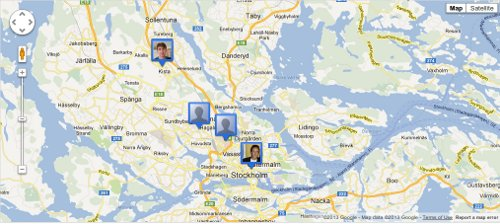
\includegraphics[scale=0.75]{context_awareness/latitude_pic.jpg}
		\caption{Figure text here} 
\end{figure}

\begin{figure}[t]
	\centering
    	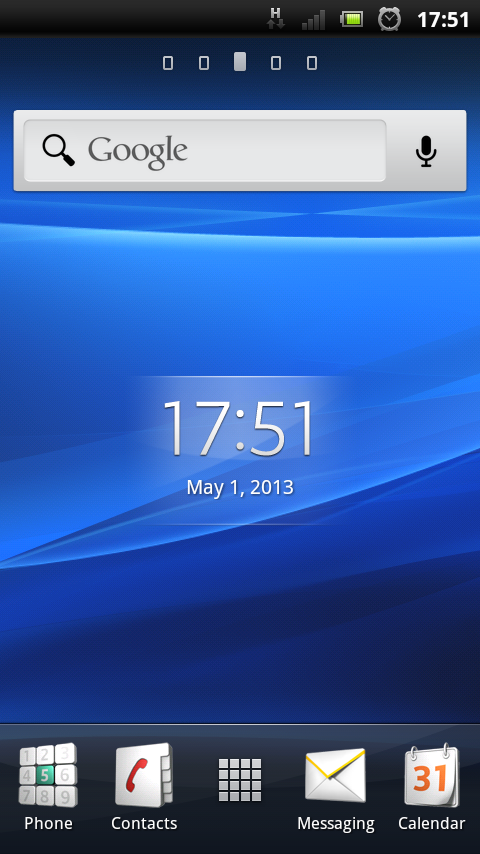
\includegraphics[scale=0.20]{context_awareness/screenshot_2013-05-01_1751.png}
    	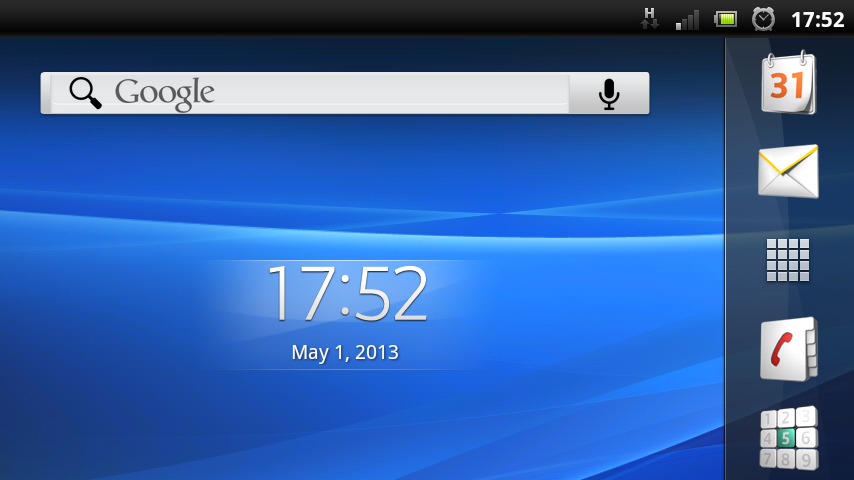
\includegraphics[scale=0.20]{context_awareness/screenshot_2013-05-01_1752.png}
		\caption{Figure text here} 
\end{figure}
	
A basic scenario of how a developer can build context\slash aware application is when the developer wants to create an application for turning on the light at home. The developer chooses to create the application without using context information. Then users will turn on lamps when pressing a button on the application. If the developer instead uses the context information the application can interact on information from sensors around the user. For example when a user enters his home the light will be turned on when the application detects his location from the users phone. The developer can also use information that provides how the weather is outside, if it's sunny outside the application will act to this and it will not turn on the lights when the user enters his home, but if it's cloudy outside the application will turn on the light.


    \backmatter
    % References
    % No restriction is set to the reference styles
    % Save your references in References.bib

    \urlstyle{same}         
    % Uncomment the line above to make urls have the same font and
    % size as the surrounding text. 

    \bibliographystyle{plain}
    \bibliography{References}

    \finalpageDSV

\end{document}